\documentclass[a4paper]{article}
%\documentclass[a4paper,fontsize=13pt]{scrartcl}

\author{Huỳnh Sâm Hà - 1610852@hcmut.edu.vn}

\usepackage{vntex}
%\usepackage{helvet} %set font Helvetica
%\usepackage{times} %set font Times New Roman
\renewcommand{\familydefault}{\sfdefault} %set font Sans Serif

%%%%% change language vietname - english
%\usepackage[english,vietnam]{babel}
%\usepackage[utf8]{inputenc}
%\usepackage[francais]{babel}

\usepackage{a4wide,amssymb,epsfig,latexsym,array,hhline,fancyhdr}
\usepackage{amsmath}
\usepackage{amsthm}
\usepackage{multicol,longtable,amscd}
\usepackage{diagbox} %Make diagonal lines in tables
\usepackage{booktabs}
\usepackage{alltt}
\usepackage[framemethod=tikz]{mdframed} % For highlighting paragraph backgrounds
\usepackage{caption,subcaption}
\usepackage{lastpage}
\usepackage[lined,boxed,commentsnumbered]{algorithm2e}
\usepackage{enumerate}
\usepackage{color}
\usepackage{graphicx} % Standard graphics package
\usepackage{array}
\usepackage{tabularx, caption}
\usepackage{multirow}
\usepackage{rotating}
\usepackage{graphics}
\usepackage[left=2.5cm,right=2.5cm,top=2cm,bottom=3cm]{geometry} % margin page
\usepackage{a4wide,amssymb,epsfig,latexsym,array,hhline,fancyhdr}
\usepackage[makeroom]{cancel}
\usepackage{arydshln}
\usepackage{textcomp}
\usepackage{listings}
\usepackage{listingsutf8}
\usepackage{verbatim}
\usepackage{setspace}

\usepackage{epsfig}
\usepackage{tikz}
\usetikzlibrary{calc}
\newcommand\HRule{\rule{\textwidth}{1pt}}
\usetikzlibrary{arrows,snakes,backgrounds}
\usepackage[unicode]{hyperref}
\hypersetup{urlcolor=blue,linkcolor=black,citecolor=black,colorlinks=true} 
%\usepackage{pstcol} % PSTricks with the standard color package

\setlength\dashlinedash{1.5pt}
\setlength\dashlinegap{4.5pt}
\setlength\arrayrulewidth{0.2pt}

% Typesetting Listings
\usepackage{xcolor}
\usepackage{color}
\definecolor{listinggray}{gray}{0.9}
\definecolor{lbcolor}{rgb}{0.9,0.9,0.9}
\definecolor{Darkgreen}{rgb}{0.1,0.6,0.1}
\definecolor{whitesmoke}{rgb}{0.99, 0.99,0.99}

\lstset{
	backgroundcolor=\color{whitesmoke},
	tabsize=2,
	language=[GNU]C++,
	basicstyle=\scriptsize,
	upquote=true,
	aboveskip={1.5\baselineskip},
	columns=fixed,
	showstringspaces=false,
	extendedchars=false,
	breaklines=true,
	prebreak = \raisebox{0ex}[0ex][0ex]{\ensuremath{\hookleftarrow}},
	frame=single,
	numbers=left,
	showtabs=false,
	showspaces=false,
	showstringspaces=false,
	identifierstyle=\ttfamily,	
	keywordstyle=\color[rgb]{0,0,1},
	commentstyle=\color[rgb]{0.026,0.112,0.095},
	stringstyle=\color[rgb]{0.627,0.126,0.941},
	numberstyle=\color[rgb]{0.205, 0.142, 0.73},
	%\lstdefinestyle{C++}{language=C++,style=numbers}’.
}
\lstset{
	backgroundcolor=\color{whitesmoke},
	tabsize=2,
	language=C++,
	captionpos=b,
	frame=lines,
	numbers=left,
	numberstyle=\tiny,
	numbersep=5pt,
	breaklines=true,
	showstringspaces=false,
	basicstyle=\footnotesize,
	%identifierstyle=\color{magenta},
	keywordstyle=\color[rgb]{0,0,1},
	commentstyle=\color{Darkgreen},
	stringstyle=\color{red}
}






\setlength{\headheight}{40pt}
\pagestyle{fancy}
\fancyhead{} % clear all header fields
\fancyhead[L]{
	\begin{tabular}{rl}
		\begin{tabular}{l}
			\textbf{Ho Chi Minh University of Technology - 
				Faculty of Computer Science \& Engineering}\\
		\end{tabular} 	
	\end{tabular}
}
\fancyhead[R]{
	\begin{tabular}{l}
		\tiny \bf \\
		\tiny \bf 
\end{tabular}  }
\fancyfoot{} % clear all footer fields
\fancyfoot[L]{\footnotesize Operating Systems - Assignment 2 - Simple Operating System}
\fancyfoot[R]{\footnotesize Trang {\thepage}/\pageref{LastPage}}
\renewcommand{\headrulewidth}{0.1pt}
\renewcommand{\footrulewidth}{0.1pt}

\setcounter{secnumdepth}{4}
\setcounter{tocdepth}{3}
\makeatletter
\newcounter {subsubsubsection}[subsubsection]
\renewcommand\thesubsubsubsection{\thesubsubsection .\@alph\c@subsubsubsection}
\newcommand\subsubsubsection{\@startsection{subsubsubsection}{4}{\z@}%
	{-3.25ex\@plus -1ex \@minus -.2ex}%
	{1.5ex \@plus .2ex}%
	{\normalfont\normalsize\bfseries}}
\newcommand*\l@subsubsubsection{\@dottedtocline{3}{10.0em}{4.1em}}
\newcommand*{\subsubsubsectionmark}[1]{}
\makeatother

\everymath{\color{blue}} %make in-line maths symbols blue to read/check easily

\sloppy
\captionsetup[figure]{labelfont={small,bf},textfont={small,it},belowskip=-1pt,aboveskip=-9pt}
%space remove between caption, figure, and text
\captionsetup[table]{labelfont={small,bf},textfont={small,it},belowskip=-1pt,aboveskip=7pt}
\setlength{\floatsep}{5pt plus 2pt minus 2pt}
\setlength{\textfloatsep}{5pt plus 2pt minus 2pt}
\setlength{\intextsep}{10pt plus 2pt minus 2pt}







\begin{document}

\begin{titlepage}

\begin{tikzpicture}[remember picture, overlay]
  \draw[line width = 3pt,color=blue] ($(current page.north west) + (2.2cm,-2.2cm)$) rectangle ($(current page.south east) + (-2.2cm,2.2cm)$);
   \draw[line width = 2pt,color=green] ($(current page.north west) + (2cm,-2cm)$) rectangle ($(current page.south east) + (-2cm,2cm)$);
\end{tikzpicture}
\vspace{1.5cm}
\begin{center} \large
ĐẠI HỌC BÁCH KHOA THÀNH PHỐ HỒ CHÍ MINH \\
\textbf{KHOA KHOA HỌC VÀ KỸ THUẬT MÁY TÍNH} \\
- - - - - - - - - - - - - - - - - - - - - 
\end{center}


\vspace{1cm}
\begin{figure}[h!]
\begin{center}

\includegraphics[width=3.6cm]{Images/LogoBK}
\end{center}
\end{figure}
\vspace{1cm}



\begin{center}
\begin{tabular}{c}
\multicolumn{1}{c}{\textbf{{\Huge HỆ ĐIỀU HÀNH}}}\\
\\ \hline \\
\textbf{{\Large Assignment 2}}\\
\\
\textbf{{\huge Simple Operating System}}\\
\\ \hline \\
\end{tabular}
\end{center}



\begin{table}[h]
\begin{tabular}{rrlrr}
\hspace{5cm} 
& {\large Giáo viên hướng dẫn}: & {\large Nguyễn Minh Trí} & & \\ 
& {\large Sinh viên}: & {\large 160852 - Huỳnh Sâm Hà} \\
\end{tabular}
\end{table}

\vspace{3cm}

\begin{center}
{\footnotesize Thành phố Hồ Chí Minh, 4/2018}
\end{center}

\end{titlepage}


\newpage \thispagestyle{empty} \tableofcontents
%\newpage \thispagestyle{empty} \listoftables
%\newpage \thispagestyle{empty} \listoffigures

\newpage

%%%%%%%%%%%%%%%%%%%%%%%%%%%%%%%%%%%%%%%%%%%
% set noindent all document
\setlength\parindent{0pt}
%%%%%%%%%%%%%%%%%%%%%%%%%%%%%%%%%%%%%%%%%%%

\section{Scheduler}

\subsection{Question - Priority Feedback Queue}

\vspace{0.5cm}

\textbf{QUESTION}: What is the advantage of using priority feedback queue in comparison with other scheduling algorithms you have learned?

\vspace{0.5cm}

Giải thuật Priority Feedback Queue (PFQ) sử dụng tư tưởng của một số giải thuật khác gồm giaỉ thuật Priority Scheduling - mỗi process mang một độ ưu tiên để thực thi, giải thuật Multilevel Queue - sử dụng nhiều mức hàng đợi các process, giải thuật Round Robin - sử dụng quantum time cho các process thực thi. Dưới đây là các giải thuật định thời khác đã học:

\vspace{0.5cm}

\begin{itemize}
	\item First Come First Served (FCFS)
	\item Shortest Job First (SJF)
	\item Shortest Remaining Time First (SRTF)
	\item Priority Scheduling (PS)
	\item Round Robin (RR)
	\item Multilevel Queue Scheduling (MLQS)
	\item Multilevel Feedback Queue (MLFQ)
\end{itemize}

\vspace{0.5cm}

Cụ thể, giải thuật PFQ sử dụng 2 hàng đợi là $ ready\_queue $ và $ run\_queue $ với ý nghĩa như sau:

\vspace{0.5cm}

\begin{itemize}
	\item $ ready\_queue $: hàng đợi chứa các process ở mức độ ưu tiên thực thi trước hơn so với hàng đợi $ run\_queue $. Khi CPU chuyển sang slot tiếp theo, nó sẽ tìm kiếm process trong hàng đợi này. 
	\item $ run\_queue $: hàng đợi này chứa các process đang chờ để tiếp tục thực thi sau khi hết slot của nó mà chưa hoàn tất quá trình của mình. Các process ở hàng đợi này chỉ được tiếp tục slot tiếp theo khi $ ready\_queue $ rỗi và được đưa sang hàng đợi  $ ready\_queue $ để xét slot tiếp theo.
	\item Cả hai hàng đợi đều là hàng đợi có độ ưu tiên, mức độ ưu tiên dựa trên mức độ ưu tiên của process trong hàng đợi.
\end{itemize}

\vspace{0.5cm}

\textbf{Ưu điểm của giải thuật PFQ}

\vspace{0.5cm}

\begin{itemize}
	\item Sử dụng time slot, mang tư tưởng của giải thuật RR với 1 khoảng quantum time, tạo sự công bằng về thời gian thực thi giữa các process, tránh tình trạng chiếm CPU sử dụng, trì hoãn vô hạn định.
	\item Sử dụng hai hàng đợi, mang tư tưởng của giải thuật MLQS và MLFQ, trong đó hai hàng đợi được chuyển qua lại các process đến khi process được hoàn tất, tăng thời gian đáp ứng cho các process (các process có độ ưu tiên thấp đến sau vẫn có thể được thực thi trước các process có độ ưu tiên cao hơn sau khi đã xong slot của mình).
	\item Tính công bằng giữa các process là được đảm bảo, chỉ phụ thuộc vào độ ưu tiên có sẵn của các process. Cụ thể xét trong khoảng thời gian $ t0 $ nào đó, nếu các process đang thực thi thì hoàn toàn phụ thuộc vào độ ưu tiên của chúng. Nếu có 1 process $ p0 $ khác đến, giả sử $ ready\_queue $ đang sẵn sàng, process $ p0 $ này vào hàng đợi ưu tiên và phụ thuộc vào độ ưu tiên của nó, cho dù trước đó các process khác có độ ưu tiên cao hơn đã thực thi xong, chúng cũng không thể tranh chấp với process $ p0 $ được vì chúng đang chờ trong  $ run\_queue $ cho đến khi $ ready\_queue $ là rỗi, tức $ p0 $ đã được thực thi slot của nó.
\end{itemize}

\vspace{0.5cm}

\subsection{Result - Gantt Diagrams}
\vspace{0.5cm}
\textbf{REQUIREMENT}: Draw Gantt diagram describing how processes are executed by the CPU.

\vspace{0.5cm}

\textbf{Test 0:}

\vspace{0.5cm}

\begin{figure}[tph]
	\centering
	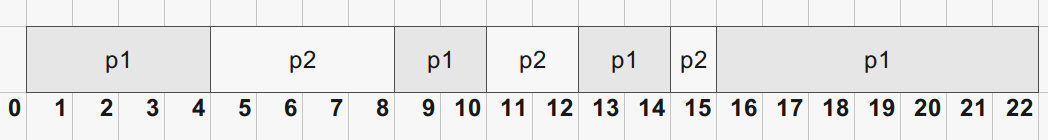
\includegraphics[width=13cm]{Images/sched0.png}
	\vspace{0.5cm}
	\caption{Lược đồ Gantt CPU thực thi các processes - test 0}
	\label{fig:schedtest0}
\end{figure}


\vspace{0.5cm}

Trong test này, CPU xử lí trên 2 process p1 và p2 trong 22 time slot như lược đồ Gantt ở trên.


\vspace{0.5cm}

\textbf{Test 1:}

\vspace{0.5cm}

\begin{figure}[tph]
	\centering
	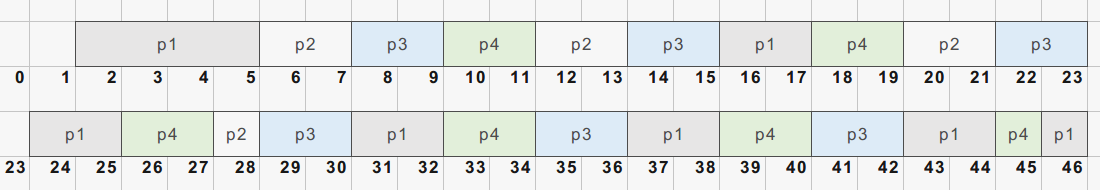
\includegraphics[width=15cm]{Images/sched1.png}
	\vspace{0.5cm}
	\caption{Lược đồ Gantt CPU thực thi các processes - test 1}
	\label{fig:schedtest1}
\end{figure}

\vspace{0.5cm}

Trong test này, CPU xử lí trên 4 process p1, p2, p3 và p4 trong 46 time slot như lược đồ Gantt ở trên.


\vspace{0.5cm}

\subsection{Implementation}
\subsubsection{Priority Queue}

Hàng đợi ưu tiên trong trường hợp này xử lý cho không quá 10 process, do đó, ta đơn giản chỉ cần dùng vòng lặp để xử lý chức năng mà một hàng đợi ưu tiên cần có.

Cụ thể với hàm  $ enqueue() $, ta chỉ cần đưa vào cuối hàng đợi nếu sẵn sàng (còn trống). Với hàm $ dequeue() $, ta duyệt tìm process có độ ưu tiên cao nhất ra, đồng thời cập nhật lại trạng thái của queue khi xóa 1 phần tử.

Dưới đây là phần hiện thực hàng đợi ưu tiên cho Scheduler.

\lstinputlisting{files/queue.c}


\subsubsection{Scheduler}

Nhiệm vụ của scheduler là quản lý việc cập nhật các process sẽ được thực thi cho CPU. Cụ thể scheduler sẽ quản lý 2 hàng đợi ready và run như ở trên đã mô tả. Trong assignment này, ta chỉ cần hiện thực tiếp hàm tìm một process cho CPU thực thi.

Cụ thể, với hàm o$ get\_proc() $, trả về một process trong hàng đợi ready, nếu hàng đợi ready rỗi, ta cấp nhật lại hàng đợi bằng các process đang chờ cho các slot tiếp theo trong hàng đợi run. Ngược lại, ta tìm ra process có độ ưu tiên cao từ hàng đợi này.

Dưới đây là phần hiện thực của chức năng nói trên.

\lstinputlisting{files/sched.c}

\section{Memory Management}

\subsection{Question - Segmentation with Paging}

\vspace{0.5cm}

\textbf{QUESTION}:What is the advantage and disadvantage of segmentation with paging?

\vspace{0.5cm}

\textbf{Ưu điểm của giải thuật}

\begin{itemize}
	\item Tiết kiệm bộ nhớ, sử dụng bộ nhớ hiệu quả.
	\item Mang các ưu điểm của giải thuật phân trang:
	\subitem Đơn giản việc cấp phát vùng nhớ.
	\subitem Khắc phục được phân mảnh ngoại.
	\item Giải quyết vấn đề phân mảnh ngoại của giải thuật phân đoạn bằng cách phân trang trong mỗi đoạn.
\end{itemize}

\vspace{0.2cm}

\textbf{Nhược điểm của giải thuật}

\begin{itemize}
	\item Phân mảnh nội của giải thuật phân trang vẫn còn.
\end{itemize}

\vspace{0.2cm}

\subsection{Result - Status of RAM}

\vspace{0.5cm}

\textbf{REQUIREMENT}: Show the status of RAM after each memory allocation and deallocation function call.

\vspace{0.5cm}


Dưới đây là kết quả của quá trình ghi log sau mỗi lệnh allocation và deallocation trong chương trình, cụ thể ghi lại trạng thái của RAM trong chương trình ở mỗi bước.


\newpage
\textbf{Test 0}:
\lstinputlisting{files/mem0.log}

\newpage
\textbf{Test 1}:
\lstinputlisting{files/mem1.log}




\subsection{Implementation}
\subsubsection{Tìm bảng phân trang từ segment}

Trong assignment này, mỗi địa chỉ được biểu diễn bởi 20 bits, trong đó 5 bits đầu tiên là segment, 5 bits tiếp theo là page, và 10 bits cuối là offset.

Chức năng này nhận vào 5 bits segment $ index $ và bảng phân đoạn $ seg\_table $, cần tìm ra bảng phân trang $ res $ của segment tương ứng trong bảng phân đoạn nói trên.

Do bảng phân đoạn $ seg\_table $ là một danh sách gồm các phần tử $ u $ có cấu trúc $ (v\_index, page\_table\_t) $, trong đó $ v\_index $ là 5 bits segment của phần tử $ u $ và $  page\_table\_t $ là bảng phần trang tương ứng của segment đó. Vì vậy để tìm được $ res $, ta chỉ cần duyệt trên bảng phân đoạn này, phần tử $ u $ nào có $ v\_index $ bằng $ index $ cần tìm, ta trả về $ page\_table $ tương ứng.

Dưới đây là phần hiện thực cho chức năng trên.

\lstinputlisting{files/getpagetable.c}


\subsubsection{Ánh xạ địa chỉ ảo thành địa chỉ vật lý}

Do mỗi địa chỉ gồm 20 bits với cách tổ chức như nói ở trên, do đó để tạo được địa chỉ vật lý, ta lấy 10 bits đầu (segment và page) nối với 10 bits cuối (offset). Mỗi $ page\_table\_t $ lưu các phần tử có $ p\_index $ là 10 bits đầu đó. do đó để tạo được địa chỉ vật lý, ta chỉ cần dịch trái 10 bits đó đi 10  bits offset rồi or (|) hai chuỗi này lại.

Dưới đây là phần hiện thực của chức năng trên.

\lstinputlisting{files/addr.c}


\newpage 
\subsubsection{Cấp phát memory}

\paragraph{Kiểm tra memory sẵn sàng}

Bước này ta kiểm tra xem memory có sẵn sàng cả trên bộ nhớ vật lý và bộ nhớ luận lí hay không.

Trên vùng vật lý, ta duyệt kiẻm tra số lượng trang còn trống, chưa được process nào sử dụng, nếu đủ số trang cần cấp phát thì vùng vật lý đã sẵn sàng. Ngoài ra để tối ưu thời gian tìm kiếm khi rơi vào trường hợp không đủ vùng nhớ, ta có thể tổ chức $ \_mem\_stat $ dưới dạng danh sách, trong đó có quản lý kích thước, vùng nhớ trống, ... để truy xuất các thông tin cần thiết nhanh chóng.

Trên vùng nhớ luận lý, ta kiểm tra dựa trên break point của process, không vượt quá vùng nhớ cho phép.

\lstinputlisting{files/memavail.c}

\paragraph{Alloc memory}

Các bước thực hiện:

\begin{itemize}
	\item Duyệt trên vùng nhớ vật lý, tìm các trang rỗi, gán trang này được process sử dụng.
	\item Tạo biến $ last\_allocated\_page\_index $ để cập nhật giá trị $ next $ dễ dàng hơn.
	\item Trên vùng nhớ luận lý, dựa trên địa chỉ cấp phát, tính từ địa chỉ bắt đầu và vị trí thứ tự trang cấp phát, ta tìm được các segment, page của nó. Từ đó cập nhật các bảng phân trang, phân đoạn tương ứng.
\end{itemize}


Dưới đây là phần hiện thực chi tiết.

\lstinputlisting{files/memalloc.c}




\subsubsection{Thu hồi memory}


\paragraph{Thu hồi địa chỉ vật lý}
Chuyển địa chỉ luận lý từ process thành  vật lý, sau đó dựa trên giá trị next của mem, ta cập nhật lại chuỗi địa chỉ tương ứng đó. 
\lstinputlisting{files/freephys.c}

\paragraph{Cập nhật địa chỉ luận lý}
Dựa trên số trang đã xóa trên block của địa chỉ vật lý, ta tìm lần lượt các trang trên địa chỉ luận lý, dựa trên địa chỉ, ta tìm được segment, page tương ứng. Sau đó cập nhật lại bảng phân trang, sau quá trình cập nhật, nếu bảng trống thì xóa bảng này trong segment đi.

\lstinputlisting{files/updv.c}

\paragraph{Cập nhật break point}
Chỉ thực hiện khi block cuối cùng trên địa chỉ luận lý được xóa, sau đó từ đó duyệt lần lượt ngược lại các trang, đến khi đến trang đang được sử dụng thì dừng.
\lstinputlisting{files/updbp.c}                   
\section{Put it all together}

Sau khi kết hợp cả scheduling và memory, ta thực hiện make all và có kết qủa như các file log trong thư mục log/os*.txt


Dưới đây là giản đồ Gantt cho trường hợp trong log/all1.txt trong source code.

\textbf{Test 0:}

\vspace{0.5cm}

\begin{figure}[tph]
	\centering
	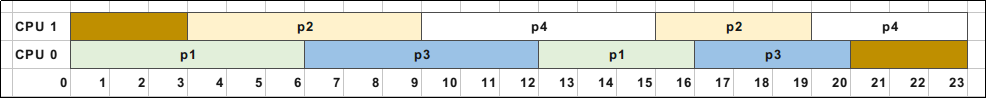
\includegraphics[width=13cm]{Images/all0.png}
	\vspace{0.5cm}
	\caption{Lược đồ Gantt CPU thực thi các processes cho make all}
	\label{fig:all0}
\end{figure}


\vspace{0.5cm}


\vspace{0.5cm}

\textbf{Test 1:}

\vspace{0.5cm}

\begin{figure}[tph]
	\centering
	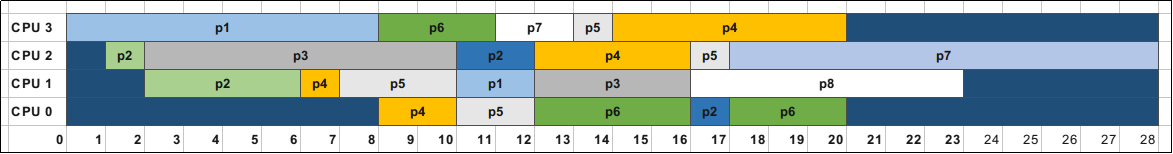
\includegraphics[width=15cm]{Images/all1.png}
	\vspace{0.5cm}
	\caption{Lược đồ Gantt CPU thực thi các processes cho make all}
	\label{fig:all1}
\end{figure}

\vspace{0.5cm}

\newpage


%%%%%%%%%%%%%%%%%%%%%%%%%%%%%%%%%
\addcontentsline{toc}{section}{Tài liệu tham khảo}
\begin{thebibliography}{99999}

% \bibitem[medium.freecodecamp.org]{medium.freecodecamp.org} {
%\href{https://medium.freecodecamp.org/building-and-installing-the-latest-linux-kernel-from-source-6d8df5345980}{How to build and install the latest Linux kernel from source?}}

\end{thebibliography}



 
\end{document}

